%!TEX root = main.tex

\documentclass[../main.tex]{subfiles}

\begin{document}

\chapter{Verification Of Slide Model and Constituent Components}

In the following chapter the testing methods used to verify the correctness of the synthesis algorithm will be detailed. As an overall strategy, the various function blocks (i.e. integer delay lines, filters) were verified first before being integrated into the larger constituent components (i.e. noise generators, string digital waveguides) which make up the synthesis model itself. The lower-level components will be introduced first as they are what the higher-level objects are built from. The objects are also roughly organized according to where they appear in the model. For instance, the constituent Control Signal Processor objects are grouped together. Filters are an exception to this rule. Full details of the testing scenarios described can be found in the attached code of the Appendix.

\section{Filters}
All the filters implemented using a class built around MATLAB's \emph{filter()} function. The general strategy for verifying correct operation of the filters is ensuring their frequency response or impulse response is correct. An exception to this rule is the Loop Filter, which will be explained in more detail in its corresponding section.

\subsection{Resonator}
As a test, the second-order resonator class was configured with the following parameters: $F_s = 48,000 \text{ Hz}$, $f_c = 5,000 \text{ Hz}$ and $r = .99$. This is illustrated below in Fig.~\ref{fig:ResoTest}.

\begin{figure}[h]
    \centering
    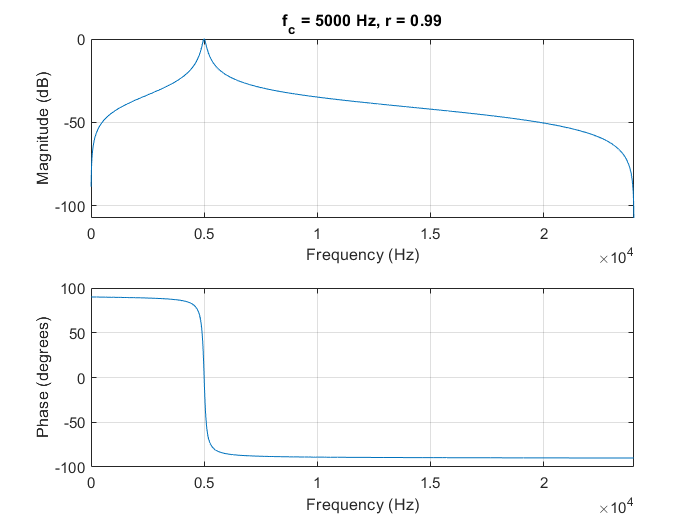
\includegraphics[scale=.65]{./images/plots/ResonatorTest.png}
    \caption{Frequency response for 2nd-order resonator test}
    \label{fig:ResoTest}
\end{figure}

\subsection{DC Blocker}
Figure~\ref{fig:DCBlockerResponse} illustrates the DC blocker's frequency response for a value of $R = .995$.

\begin{figure}[h]
    \centering
    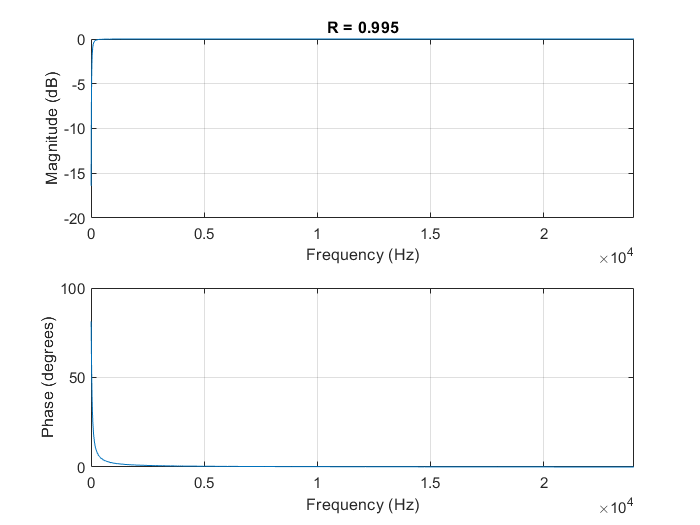
\includegraphics[scale=.65]{./images/plots/DCBlockerResponse.png}
    \caption{DC Blocker Frequency Response}
    \label{fig:DCBlockerResponse}
\end{figure}

\clearpage

\subsection{Longitudinal Modes}
The precise method by which the longitudinal mode filters were derived and designed is not completely specified in either \citetwo{puputti_real-time_2010} or \citetwo{pakarinen_virtual_2008}. What is explained is that a linear-prediction filter of order 100 was used to estimate the spectrum of the different modes of each slide/wound string interaction. From this a 4th-order IIR filter was derived based on the most prominent resonances. The pole/zero locations for these 4th-order filters are what is provided for an implementation. Magnitude responses for the different filters as well as the linear-prediction estimates are provided as shown in Fig.~\ref{fig:LongModeOrig}. These plots for the 4th-order approximations were recreated for the implemented longitudinal mode filters as shown in Fig.~\ref{fig:LongModeRecr}. Verification was done through visual comparison of the plots as it was the best option available.

\subsection{Smoothing Filter}
The smoothing filters is implemented via a 10-point moving average where every sample is weighted evenly. Accordingly, it is expected that the impulse response will be 10 impulses all scaled by $\frac{1}{10}$ as the impulse response of an FIR is the same as its coefficients. This is verified by the output shown in Fig.~\ref{fig:SmoothingIR}. Extra elements are shown to indicate the filter outputs zeros after the 10th iteration (corresponding to $n = 9$). Given that it is easier to understand this filter from its impulse response, and this is is paired to the frequency response via the Fourier Transform, verification for this was done in the time-domain.

\begin{figure}[h]
    \centering
    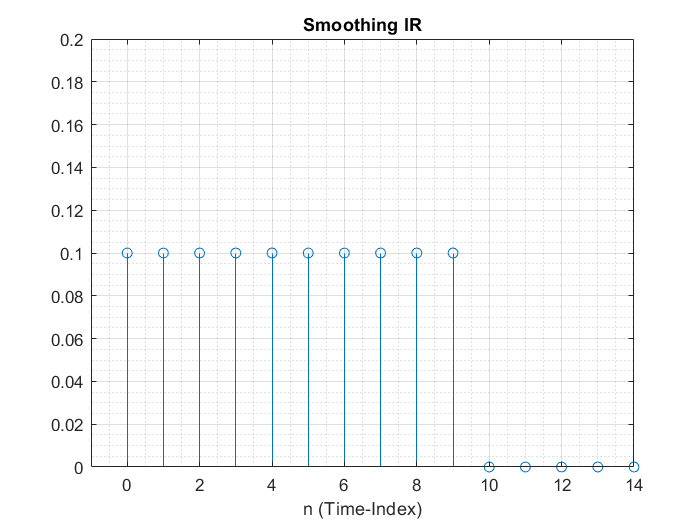
\includegraphics[scale=.65]{./images/plots/SmoothingIR.png}
    \caption{Verification for smoothing filter}
    \label{fig:SmoothingIR}
\end{figure}

\begin{figure}[h]
        \centering
        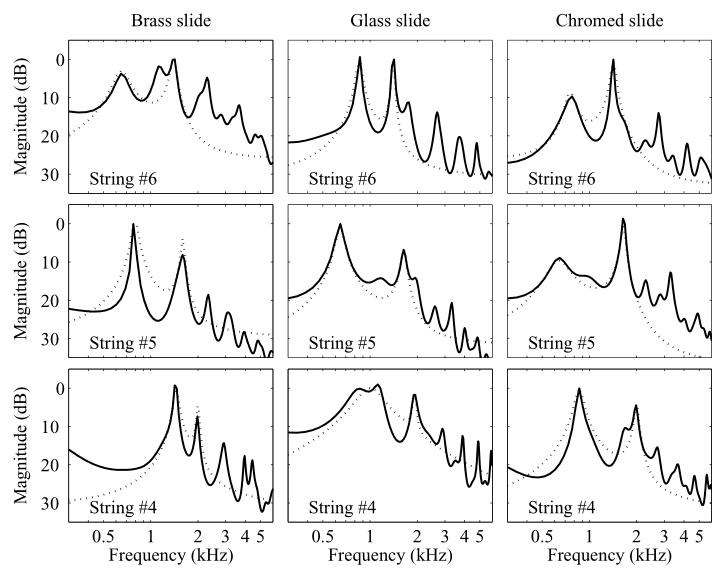
\includegraphics[scale=.65]{./images/plots/LongitudinalModeFiltersOriginal.png}
        \caption{Original figure from \citetwo{pakarinen_virtual_2008} for comparison purposes. Solid lines represent spectral estimates using linear-prediction filter of order 100. Dashed lines indicate modal filter magnitude responses.}
        \label{fig:LongModeOrig}
\end{figure}

\begin{figure}[h]
        \centering
        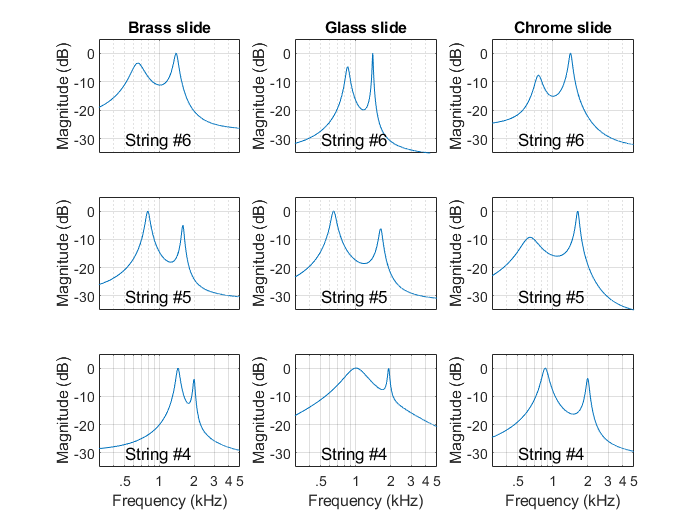
\includegraphics[scale=.65]{./images/plots/LongitudinalModeFiltersRecreation.png}
        \caption{Plot of the different contact sound filter responses for modal filters.}
        \label{fig:LongModeRecr}
\end{figure}

\clearpage

\section{CSP and Components}
\subsection{Components}
\subsubsection{Interpolator}
The interpolator block operates via linear interpolation. It was tested by specifying a control signal $L[m]$ and running it through the interpolator. The original $L[m]$ was plotted with linear line segments connecting between the points. The interpolated $L[n]$ output was plotted as individual samples overlaid onto the original to ensure that the linear trajectories were maintained. Figure~\ref{fig:InterpTest} illustrates this. For this figure, the audio rate was specified as 48,000 Hz while the control rate was specified as 12,000 Hz. This would give a ratio of $R = \frac{48000}{12000} = 4$, meaning 3 interpolated audio samples would need to be calculated for every 1 control sample. The black dashed lines in the figure correspond to the boundaries between the interpolation frames. It is also necessary to specify an initial value for the interpolation to start from. In this figure $.5$ was used.

\begin{figure}[h]
    \centering
    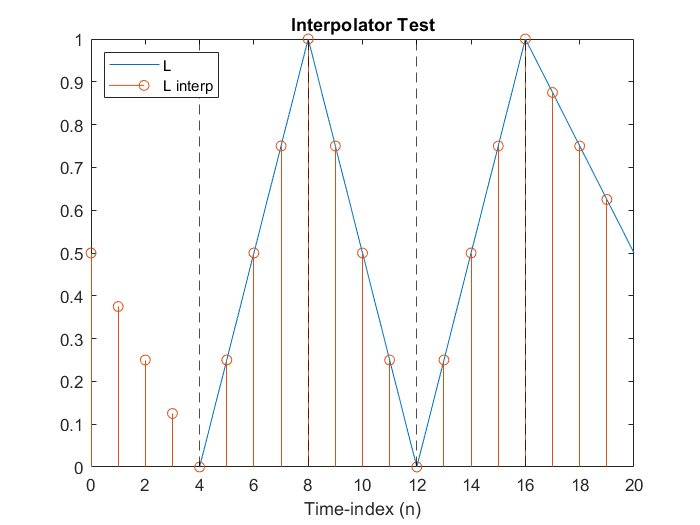
\includegraphics[scale=.65]{./images/plots/InterpolatorTest.png}
    \caption{Output from Interpolator test. Red line segments have been added to help illustrate the linearity. The initial value used to start the interpolation from is .5 and R = 4.}
    \label{fig:InterpTest}
\end{figure}

\subsubsection {Slide Speed Extractor}
The Slide Speed Extractor was tested by taking a theoretical curve which represents a parabolic $slideSpeed[n]$ trajectory. From this, the corresponding relative length signal for a specified string length was generated using the equation:
\begin{equation}
    L[n] = L[n-1] - \frac{slideSpeed[n]}{F_s \times StringLength}
\end{equation}
This curve was then fed into the Slide Speed Extractor object to generate the corresponding $slideSpeed[n]$. The error between the theoretical and measured values was calculated. The output of this is shown in Fig.~\ref{fig:SlideSpeedTest}.

\begin{figure}[h]
    \centering
    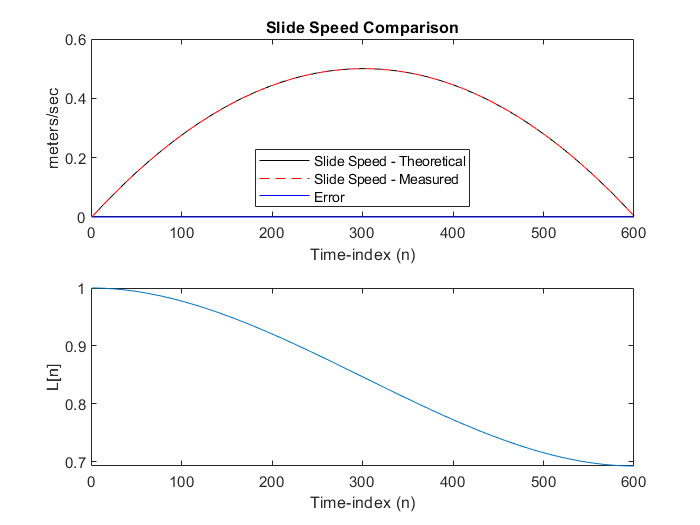
\includegraphics[scale=.65]{./images/plots/SlideSpeedExtractorTest.png}
    \caption{The top plot illustrates the correctness of the slide speed extraction algorithm while the lower plot displays the $L[n]$ signal which was used as a stimuli.}
    \label{fig:SlideSpeedTest}
\end{figure}

\subsection{Control Signal Processor}
With the constituent components verified as working, the test here confirms that everything is linked together correctly inside the Control Signal Processor. Figure~\ref{fig:CSPTest} illustrates the output of the Control Signal Processor to a specified $L[m]$ control signal. This was chosen to be linear to make the interpolation and smoothing easier to verify. The $slideSpeed[n]$ signal can be seen as indicating the slide starts from rest and then gradually ramps up to constant speed. This is consistent with what would be expected as we have specified that the starting $L[m]$ value in the CSP corresponds to when $m = 0$.

\clearpage

\begin{figure}[h]
    \centering
    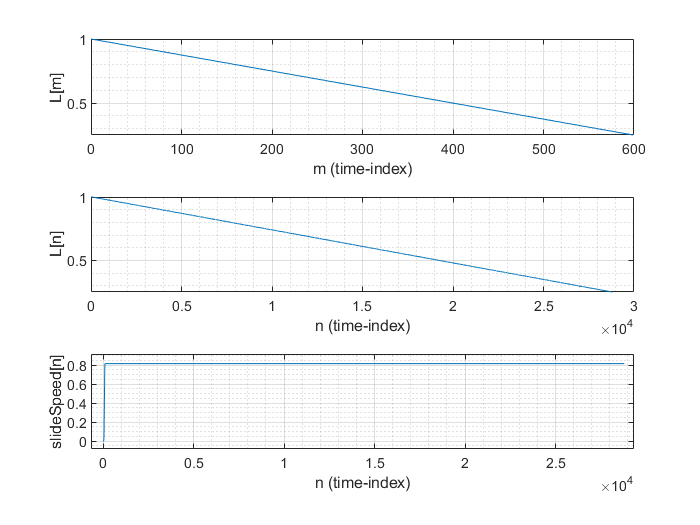
\includegraphics[scale=.65]{./images/plots/CSPTest.png}
    \caption{$L[m]$ input signal and corresponding output signals for CSP test}
    \label{fig:CSPTest}
\end{figure}

\subsection{Loop Filter}
As described before, the loop filter was designed to approximate the various losses associated with vibrating string motion. It is a a simple one-pole filter which uses a first-order polynomial approximation to generate $a$ and $g$ coefficients at various relative string length values (as described in the introduction chapter). Limitations of this approach have been shown which illustrated that the filter itself is operational through examining its various frequency response characteristics. The original paper provides the equations for the polynomial approximation as well as the polynomial coefficients. No frequency response plots are provided. In terms of the polynomial approximation, results are only provided for the first string. Accordingly the verification approach here involves recreating the original figures and relying on the fact the other coefficients have been copied correctly. Figure~\ref{fig:Fig18Orig} and Fig.~\ref{fig:Fig19Orig} show the original plots while Fig.~\ref{fig:Fig18Recon} and Fig.~\ref{fig:Fig19Recon} show the recreations respectively.

\begin{figure}[h]
    \centering
    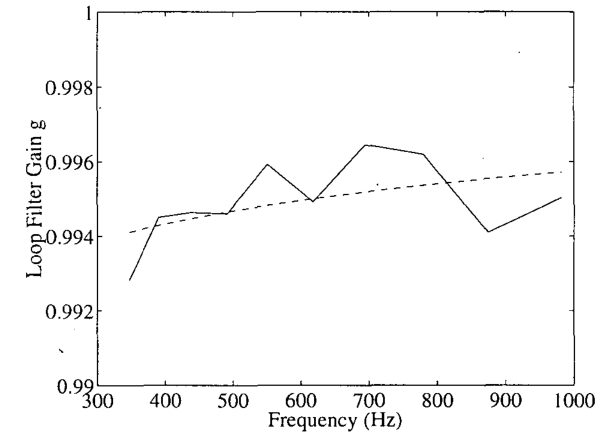
\includegraphics[scale=.75]{./images/plots/Figure18Orig.png}
    \caption{Loop gain \emph{g} for modeling string 1 (solid line) and first-order polynomial fit (dashed line) from \citetwo{valimaki_development_1998}}
    \label{fig:Fig18Orig}
\end{figure}

\begin{figure}[h]
    \centering
    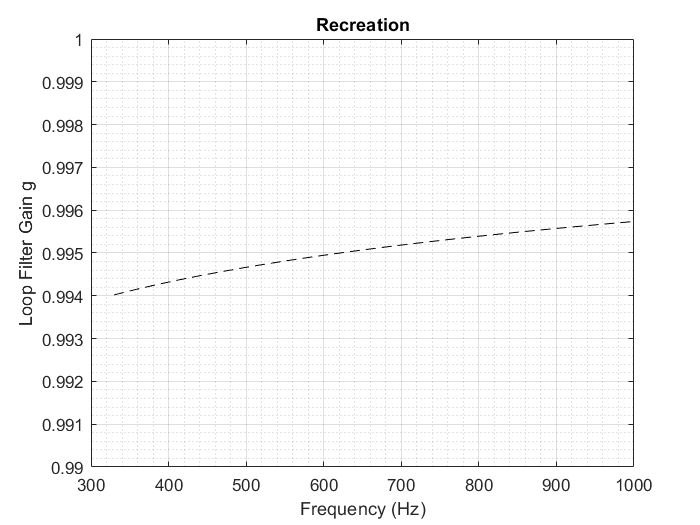
\includegraphics[scale=.65]{./images/plots/Figure18Recon.png}
    \caption{Loop gain \emph{g} polynomial for string 1}
    \label{fig:Fig18Recon}
\end{figure}

\begin{figure}[h]
    \centering
    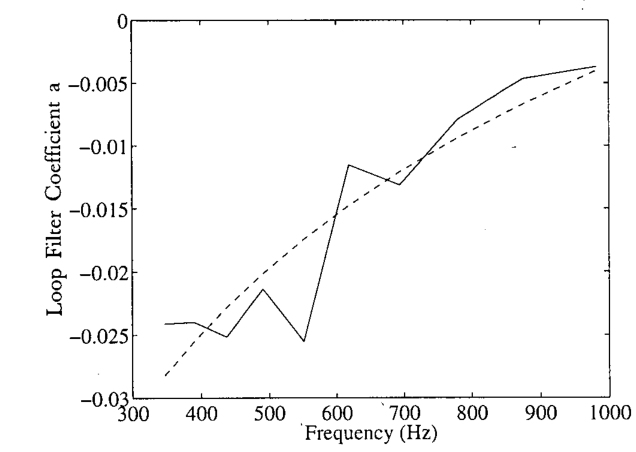
\includegraphics[scale=.75]{./images/plots/Figure19Orig.png}
    \caption{Loop-filter \emph{a} for string 1 (solid line) and first-order polynomial fit (dashed line) from \citetwo{valimaki_development_1998}}
    \label{fig:Fig19Orig}
\end{figure}

\begin{figure}[h]
    \centering
    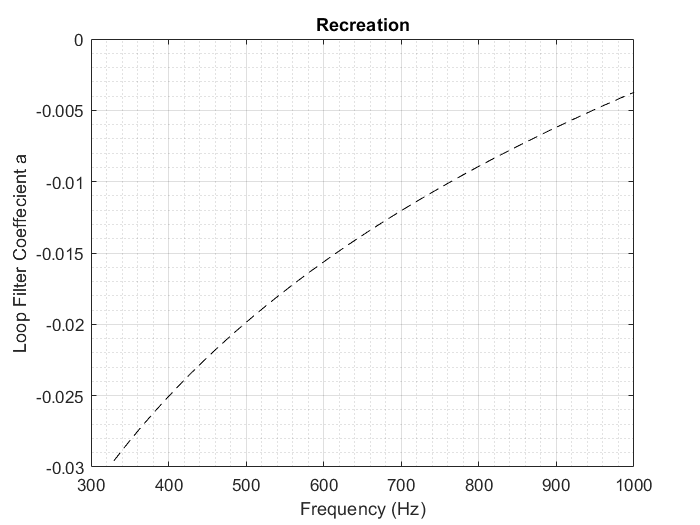
\includegraphics[scale=.65]{./images/plots/Figure19Recon.png}
    \caption{Loop-filter \emph{a} polynomial for string 1}
    \label{fig:Fig19Recon}
\end{figure}

\clearpage

\section{Noise Generation Objects}
\subsection{Impulse Train}
The Impulse Train object responds to the $f_c[n]$ signal which controls its firing rate. Accordingly, various artificial $f_c[n]$ signals were generated to ensure the different run-time use cases would execute correctly during synthesis. Figure~\ref{fig:ImpulseTrainTest} provides a summary of the tests and output. The full details can be found in the Appendix. 

\begin{figure}[h]
    \centering
    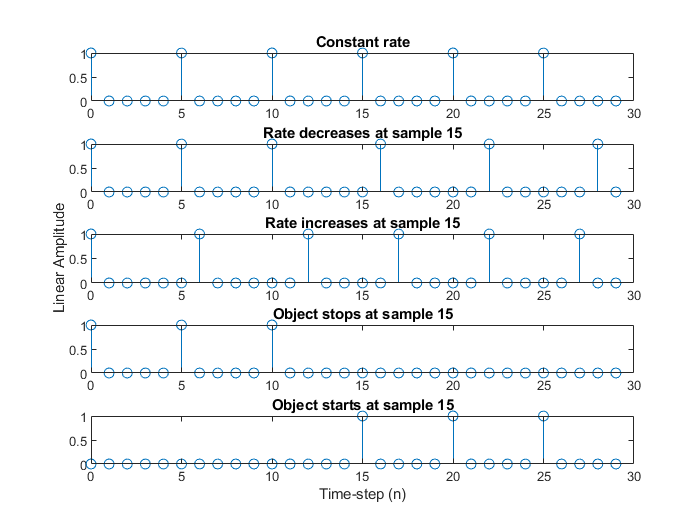
\includegraphics[scale=.65]{./images/plots/ImpulseTrainTest.png}
    \caption{Impulse Train test output}
    \label{fig:ImpulseTrainTest}
\end{figure}

\subsection{Exponential Decay}
The Exponential Decay object is composed of a Impulse Train fed into a one-pole IIR filter whose feedback coefficient is tuned to match the specified $T_{60}$ parameter. As the Impulse Train was tested separately, it was necessary to ensure that the $T_{60}$ parameter was implemented correctly. Figure~\ref{fig:ExpDecayTest1} illustrates correct functioning of the object for three different $T_{60}$ values where they have been converted from seconds to samples. 

\begin{figure}[ht]
    \centering
    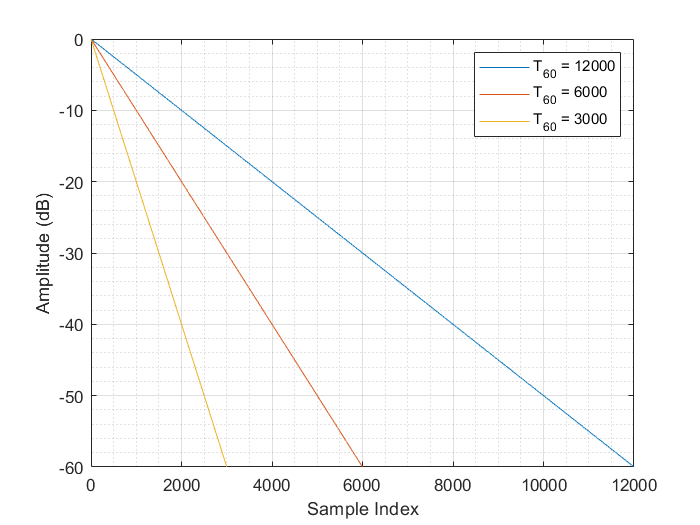
\includegraphics[scale=.55]{./images/plots/ExpDecayTest1.png}
    \caption{Test results for different $T60$ decay parameters specified in samples}
    \label{fig:ExpDecayTest1}
\end{figure}
 
\subsection{Noise Pulse Train}
The Noise Pulse Train object was tested with two different scenarios: a constant firing rate producing 12 distinct pulses with no overlap and an swept firing rate corresponding to the same parabolic trajectory used in previous tests. The results are illustrated in Fig.~\ref{fig:NPTT1}, Fig.~\ref{fig:NPTT2} and Fig.~\ref{fig:NPTT2Spec}. Note the overlap of the individual pulses in the second test due to the firing rate being faster than the decay rate. The spectrum also illustrates how the signal has a harmonic component in the lower end. The output of each test can be heard in the files \emph{NoisePulseTrain-test1.wav} and \emph{NoisePulseTrain-test2.wav}. The ``noisiness" of a signal at higher values of $f_c$ can be controlled by the $T_{60}$ parameter as will be discussed in the Sound Design chapter.

\begin{figure}[h!]
    \centering
    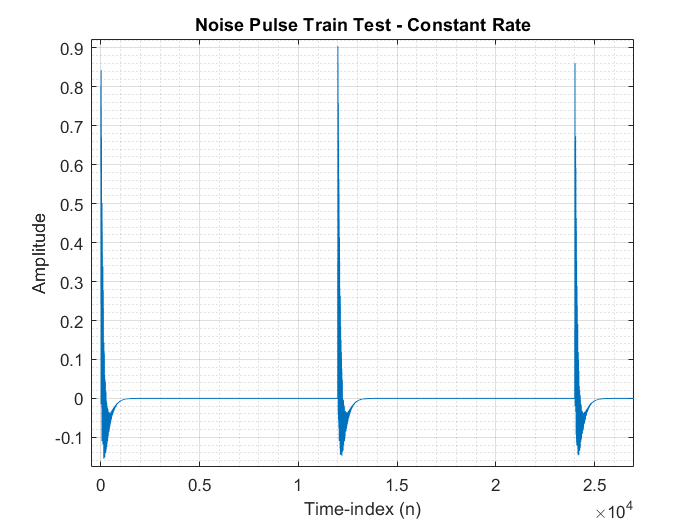
\includegraphics[scale=.55]{./images/plots/NPTTest1.png}
    \caption{Noise Pulse Train output for a constant rate. Note the negative values introduced by the DC Blocker.}
    \label{fig:NPTT1}
\end{figure}

\clearpage

\begin{figure}[t]
    \centering
    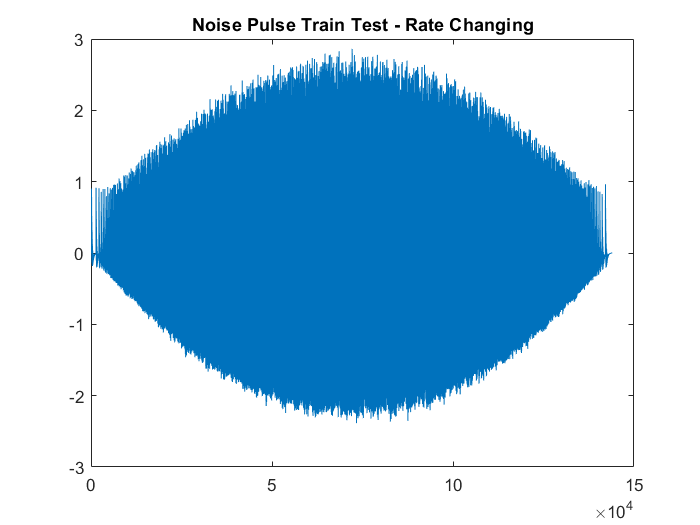
\includegraphics[scale=.65]{./images/plots/NPTTest2.png}
    \caption{Noise Pulse Train output in response to an $f_c[n]$ sweep. Note the overlapping build-up of the individual impulses. Individual pulses can be seen at the ends.}
    \label{fig:NPTT2}
\end{figure}

\begin{figure}[b]
    \centering
    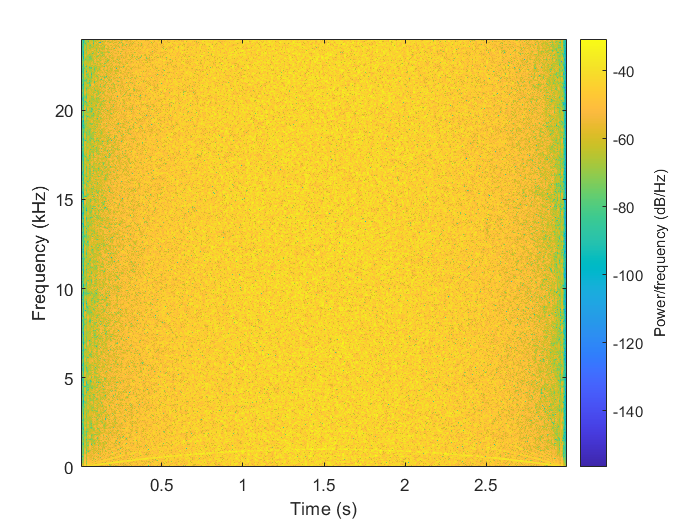
\includegraphics[scale=.65]{./images/plots/NPTTest2Spectrum.png}
    \caption{Spectrum corresponding to Fig.~\ref{fig:NPTT2}. Note the emergence of harmonics at the lower end.}
    \label{fig:NPTT2Spec}
\end{figure}

\clearpage

\subsection{Noise Burst Generator}
\label{sec:NBGVerify}
The Noise Burst generator was tested with the same two scenarios as the Noise Pulse Train. The outputs are shown in Fig.~\ref{fig:NBGT1}, Fig.~\ref{fig:NBGT2} and Fig.~\ref{fig:NBGT2Spec}. The sounds can be heard in the files \emph{NoiseBurstGen-test1.wav} and \emph{NoiseBurstGen-test2.wav}. The noisiness in the second example was by design as explained in Chapter 3. Each of the different noise sources were originally designed to work with a different Harmonic Accentuation technique. The Noise Burst Generator pairs best with the Harmonic Resonator Bank.

\begin{figure}[hb]
    \centering
    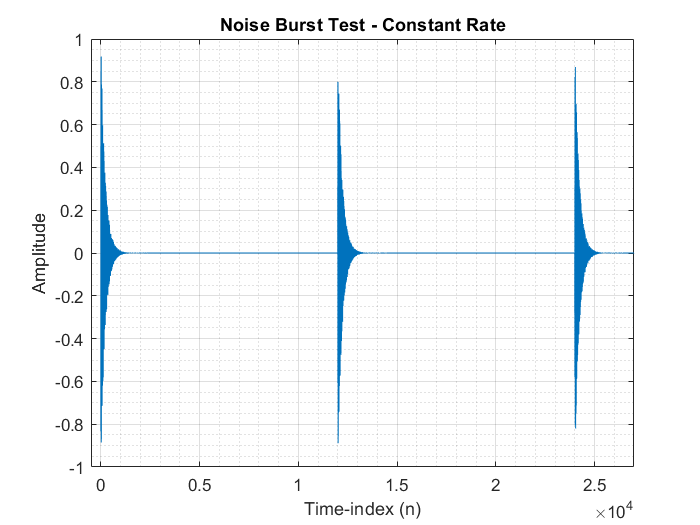
\includegraphics[scale=.65]{./images/plots/NBGTest1.png}
    \caption{Noise Burst Generator output for a constant rate. Note the approximate symmetry about the x-axis.}
    \label{fig:NBGT1}
\end{figure}

\begin{figure}[ht]
    \centering
    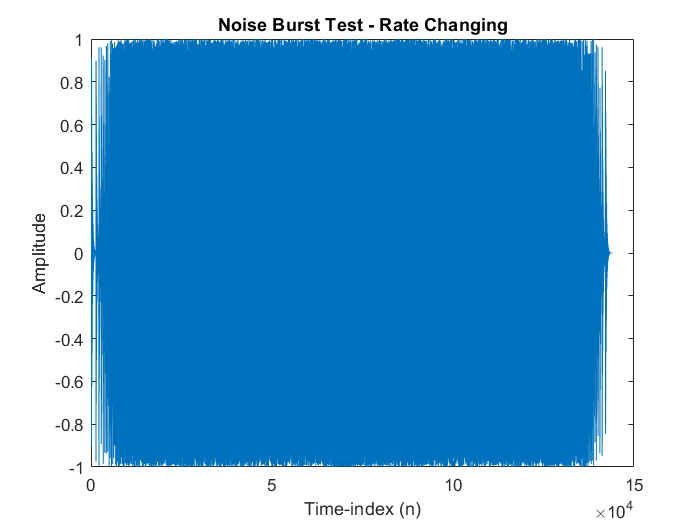
\includegraphics[scale=.65]{./images/plots/NBGTest2.png}
    \caption{Noise Burst Generator output in response to an $f_c[n]$ sweep. Note the effects of the hard-clipping.}
    \label{fig:NBGT2}
\end{figure}

\begin{figure}[hb]
    \centering
    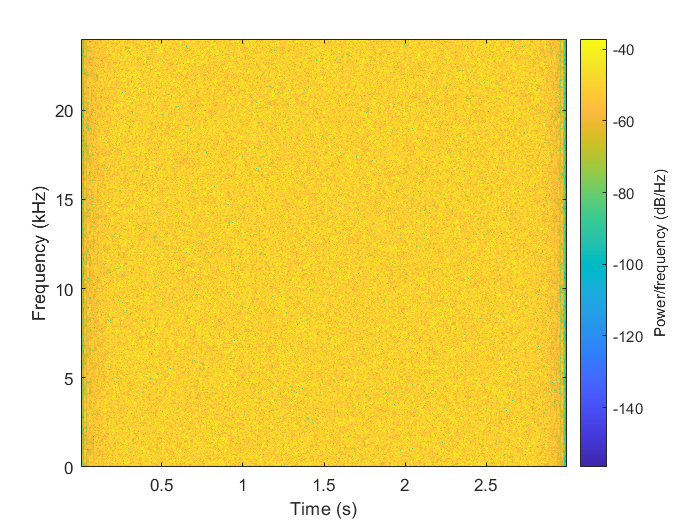
\includegraphics[scale=.65]{./images/plots/NBGTest2Spectrum.png}
    \caption{Spectrum corresponding to Fig.~\ref{fig:NBGT2}. Note the lack of harmonics.}
    \label{fig:NBGT2Spec}
\end{figure}

\clearpage

\section{Harmonic Accentuators}
\subsection{Harmonic Resonator Bank}
Given that the resonators were tested already, the Harmonic Resonator Bank was verified by running white noise through the system while performing a sweep on the $f_c$ control parameter. The sweep follows the same parabolic trajectory as before. The functionality of this block predicts that we would observe six harmonically linked bands in the output spectrum. This is shown in Fig.~\ref{fig:HRBTest} where the different harmonics' trajectories are overlaid in red. The output can be heard in \emph{HRB-test.wav}.

\begin{figure}[h]
    \centering
    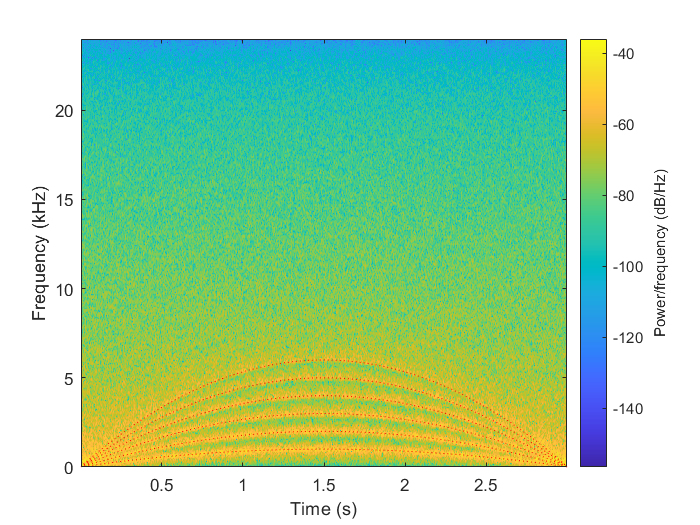
\includegraphics[scale=.65]{./images/plots/HRBTest.png}
    \caption{Output from Harmonic Resonator Bank test}
    \label{fig:HRBTest}
\end{figure}

\subsection{Reso + Tanh}
The Reso + Tanh block was tested using the same $f_c$ sweep. The stimuli was changed to use the Noise Pulse Train object instead as the $\tanh()$ function relies on a harmonic signal being input in order to achieve the desired effect of accentuating/creating harmonics. Figure~\ref{fig:ResoTanhTest} illustrates the output spectrum from the test. Note the much finer concentration of energy in the harmonic bands, the emphasis of the fundamental due to the different noise source and more than 6 harmonics being generated. The output of this can be heard in \emph{ResoTanh-test.wav}.

\begin{figure}[h]
    \centering
    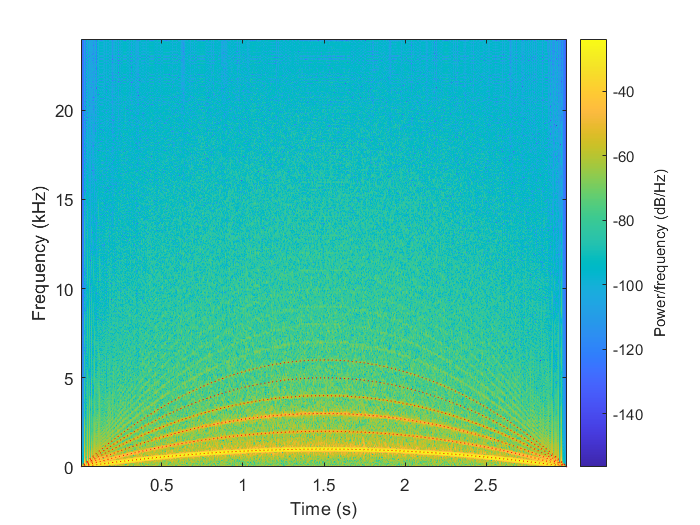
\includegraphics[scale=.65]{./images/plots/ResoTanhTest.png}
    \caption{Output from Reso + Tanh test}
    \label{fig:ResoTanhTest}
\end{figure}

\section{Contact Sound Generator}
Both the wound and unwound CSGs were verified using the following three test cases based on the qualities of the slide motion:

\begin{enumerate}
    \item No slide motion
    \item Slide motion with a constant slide velocity
    \item Slide motion with a time-varying slide velocity
\end{enumerate}

These were selected as they covered the basic use cases which would arise during synthesis. The constant slide velocity test uses a slide velocity which generates an $f_c[n]$ of 250 Hz. The time-varying slide velocity is configured to generate a parabolic sweep of $f_c[n]$ from 0 Hz to 1kHz and back to 0 Hz (as with the previous similar tests). This mimics the speed experienced by a slide which starts at rest and moves between two positions on the fingerboard. Test scenario 1 is mentioned for completeness purposes. Results and figures from that test will not be discussed due to its simplicity.

\subsection{Wound Variant}
The audio producing tests were further sub-divided into three other tests by controlling the balance between the two sound components. This was done to ensure proper functioning of each branch as well as get a sense for the audible contribution of each one in the combined sound. As part of the sound design process, the four different combinations of noise sources and harmonic accentuation techniques were tested (as will be elaborated upon in the Sound Design chapter). The following figures were generated using the Noise Pulse Train and Harmonic Resonator Branch configuration in order to reduce the total number of figures.

\begin{enumerate}
    \item Longitudinal branch isolated
    \item Harmonic branch isolated
    \item Both branches combined
\end{enumerate}

In the spectrograms showing the results, the dashed black lines represent the specified longitudinal mode frequencies and the dotted red lines indicate the theoretical harmonic trajectories.

\subsubsection{Static $f_c[n]$}
The results for the constant slide velocity scenario are shown in Fig.~\ref{fig:CSGWoundStaticLong}, Fig.~\ref{fig:CSGWoundStaticHarm} and Fig.~\ref{fig:CSGWoundStaticBoth}. Figure~\ref{fig:CSGWoundTVLong} illustrates how the original source stimuli produced by the Noise Pulse Generator does not contain strong frequency components at the 1st longitudinal mode frequency. Also illustrated is that the harmonic branch extracts and emphasizes the fundamental while retaining many of the upper harmonics in decreasing strength. The corresponding audio can be heard in \emph{CSG-Wound-Static-Long.wav}, \emph{CSG-Wound-Static-Harm.wav} and \emph{CSG-Wound-Static-Both.wav}.

\begin{figure}[h!]
    \centering
    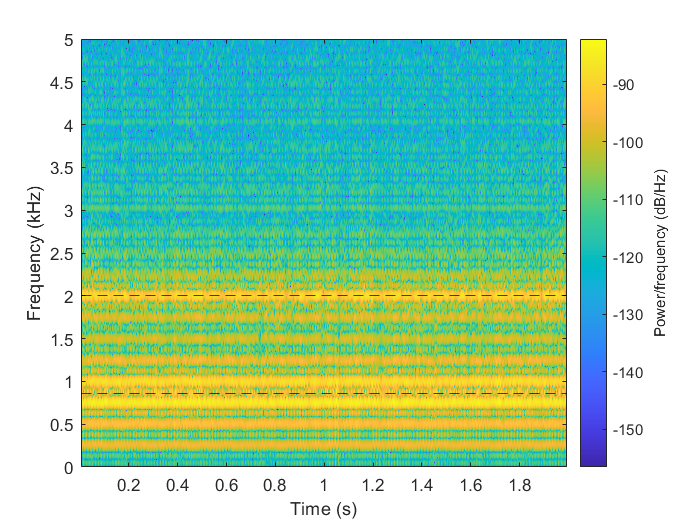
\includegraphics[scale=.58]{./images/plots/CSG_Wound_Static_Long.png}
    \caption{Output from the Wound CSG test using a static slide velocity for the longitudinal branch. The dashed black lines indicate longitudinal mode frequencies. As the stimuli doesn't contain frequencies near the first mode, there is less energy there.}
    \label{fig:CSGWoundStaticLong}
\end{figure}

\begin{figure}[t]
    \centering
    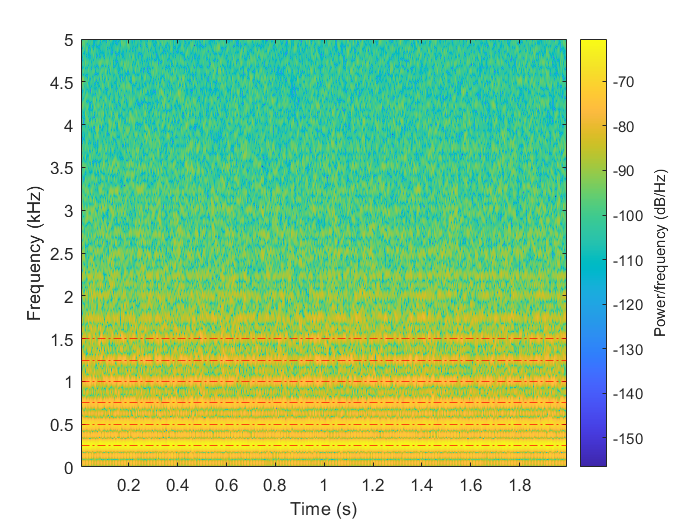
\includegraphics[scale=.60]{./images/plots/CSG_Wound_Static_Harm.png}
    \caption{Output from the Wound CSG test using a static slide velocity for the harmonic branch. The dotted red lines indicate the frequencies for the first six harmonics.}
    \label{fig:CSGWoundStaticHarm}
\end{figure}

\begin{figure}[b]
    \centering
    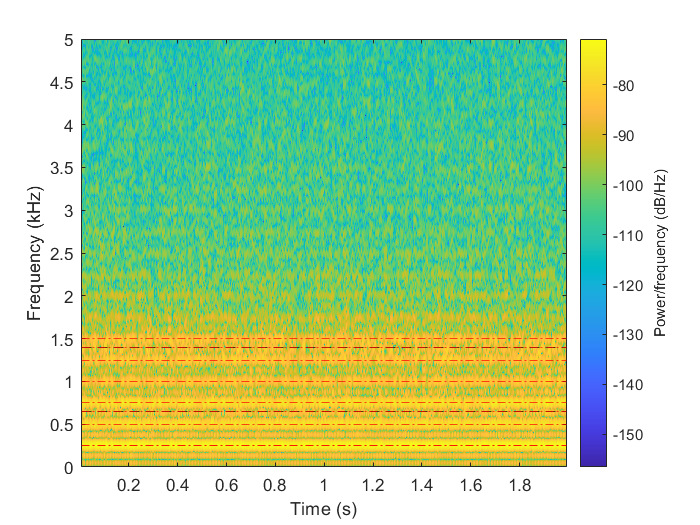
\includegraphics[scale=.60]{./images/plots/CSG_Wound_Static_Both.png}
    \caption{Output from the Wound CSG test using a static slide velocity for both combined branches. Notice how this is a combination of Fig.~\ref{fig:CSGWoundStaticLong} and Fig.~\ref{fig:CSGWoundStaticHarm}.}
    \label{fig:CSGWoundStaticBoth}
\end{figure}

\clearpage

\subsubsection{Time-Varying $f_c[n]$}
The results for the time-varying scenario are shown in Fig.~\ref{fig:CSGWoundTVLong}, Fig.~\ref{fig:CSGWoundTVHarm} and Fig.~\ref{fig:CSGWoundTVBoth}. Dashed red lines indicate the theoretical harmonic trajectories. Dashed blacked lines correspond to the static longitudinal modes. As is clearly shown in Fig.~\ref{fig:CSGWoundTVLong}, the longitudinal modes are only stimulated when the frequencies the filters are tuned to are present in the incoming signal. It also illustrates how some of the harmonic components leak through due to imperfections in the filter. Only $\frac{1}{3}$ of the spectrum is plotted to emphasize these points. The corresponding audio can be heard in \emph{CSG-Wound-TV-Long.wav}, \emph{CSG-Wound-TV-Harm.wav} and \emph{CSG-Wound-TV-Both.wav}.

\begin{figure}[hb]
    \centering
    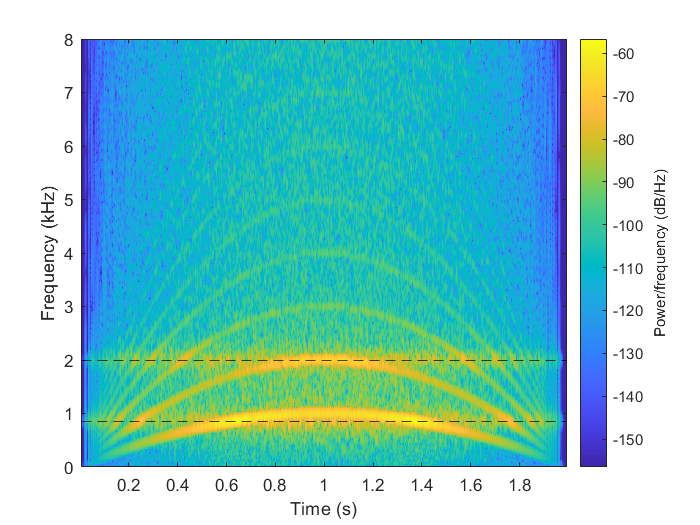
\includegraphics[scale=.65]{./images/plots/CSG_Wound_TV_Long.png}
    \caption{Output from the Wound CSG test using a time-varying slide velocity for the longitudinal branch. The dashed black lines indicate longitudinal mode frequencies. When the fundamental of the sweep matches a modal frequency it is reinforced more.}
    \label{fig:CSGWoundTVLong}
\end{figure}

\begin{figure}[t]
    \centering
    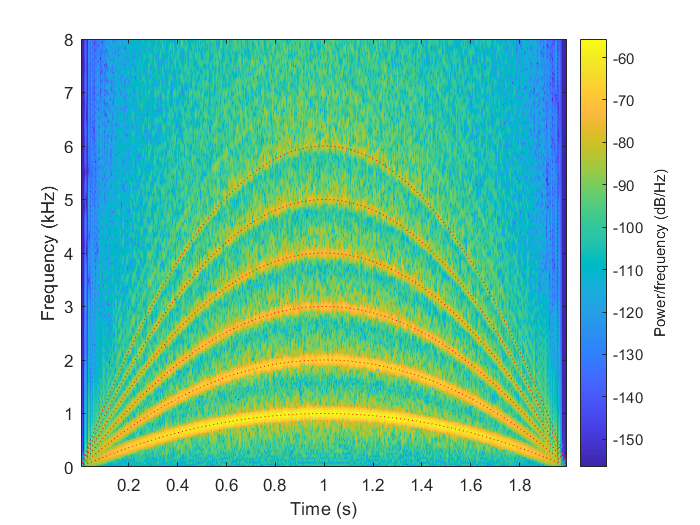
\includegraphics[scale=.60]{./images/plots/CSG_Wound_TV_Harm.png}
    \caption{Output from the Wound CSG test using a time-varying slide velocity for the harmonic branch. The dotted red lines indicate the frequencies for the first six harmonics.}
    \label{fig:CSGWoundTVHarm}
\end{figure}

\begin{figure}[b]
    \centering
    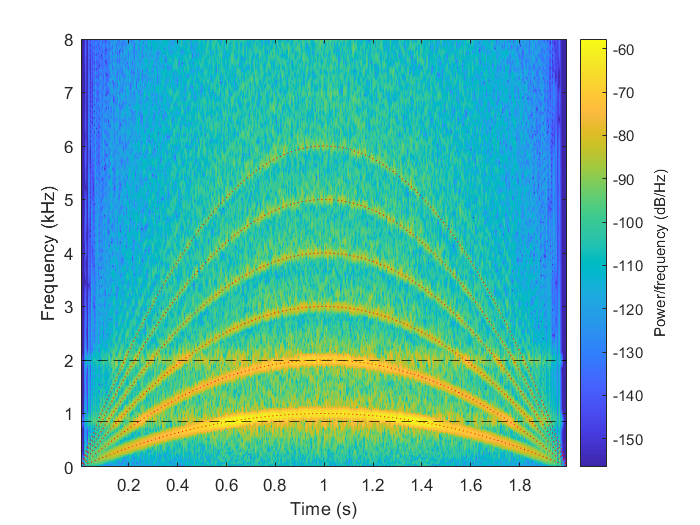
\includegraphics[scale=.60]{./images/plots/CSG_Wound_TV_Both.png}
    \caption{Output from the Wound CSG test using a static slide velocity for both combined branches. Notice how this is a combination of Fig.~\ref{fig:CSGWoundTVLong} and Fig.~\ref{fig:CSGWoundTVHarm}.}
    \label{fig:CSGWoundTVBoth}
\end{figure}

\clearpage

\subsection{Unwound Variant}
Figure~\ref{fig:CSGUnwoundTVSpec} illustrates the output of the unwound Contact Sound Generator for the same time-varying slide speed signal. It is substantially less interesting but still necessary for the purposes of verification. As can be seen the low-pass filter applied creates a roll-off at the top of the spectrum while the ramp-in and ramp-down create the variations in spectral energy near the beginning and end of the sound. This can be heard in the file \emph{CSG-Unwound-TV.wav}. The rest of the scenarios were also run on this module (as can be seen in the Appendix) but aren't shown here.

\begin{figure}[h]
    \centering
    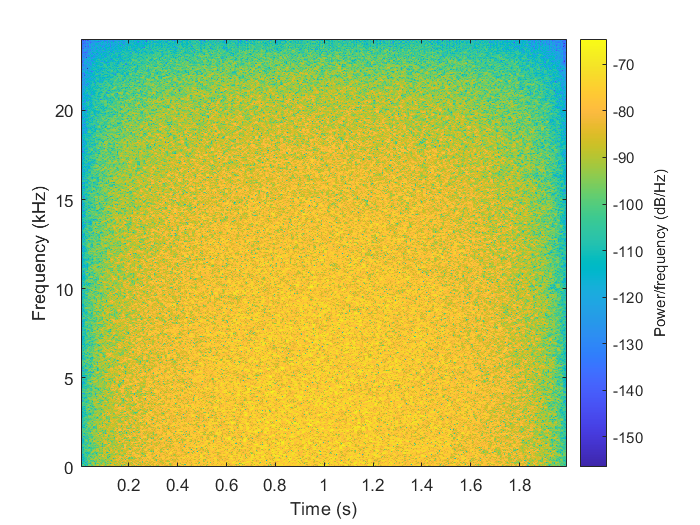
\includegraphics[scale=.65]{./images/plots/CSG_Unwound_TV.png}
    \caption{Output from unwound branch for time-varying slide velocity}
    \label{fig:CSGUnwoundTVSpec}
\end{figure}

\section{String DWG and Components}

\subsection{Interpolated Delay Line}
The core-class which this object was built around is a circular buffer. The circular buffer class was tested thoroughly itself (as will be shown in the Appendix). Illustrated here will be the verification aspects of the Lagrange interpolation as these are crucial to ensuring the correct functioning of the synthesis algorithm. In this test, $M$ represents delay in samples as implemented by the integer delay line while $D$ represents the total delay implemented by the Lagrange interpolator. $d$ is the fractional delay. $D = \lfloor D \rfloor + d$. The order of the Lagrange interpolator is set to 5.

The first test which was performed was a test to ensure that it could indeed operate as an integer delay. Various Lagrange objects were constructed, ensuring that no fractional delay would be required. The output of this test is shown in Fig.~\ref{fig:LagrangeTest1} where $x$ is the input signal and $y$ is the output. As this figure clearly shows, the interpolated delay line clearly implements this functionality.

\begin{figure}[h]
    \centering
    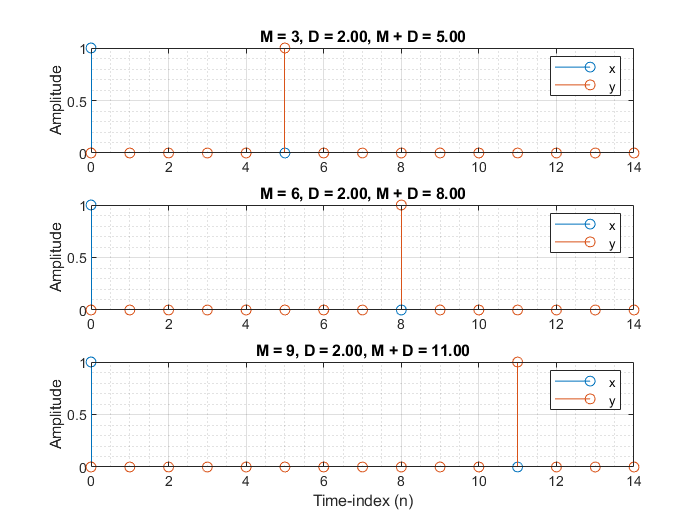
\includegraphics[scale=.65]{./images/plots/LagrangeTest1.png}
    \caption{Test results of integer values for fractional delay object. $x[n]$ is the input impulse stimuli and $y[n]$ is the resulting delayed output. The delay values are broken down above each plot.}
    \label{fig:LagrangeTest1}
\end{figure}

The second test which was performed ensures that the delay line value can be updated during the run-time. This differs from the previous test where a new object was constructed each time. Figure~\ref{fig:LagrangeTest2} illustrates this test. The delay line starts out with an initial delay of 10 samples. After 15 samples have passed this is incremented by 1. After another 15 samples have passed this is decremented by two. Impulses are fed into the delay line every 15 samples to show the changes.

\begin{figure}[h]
    \centering
    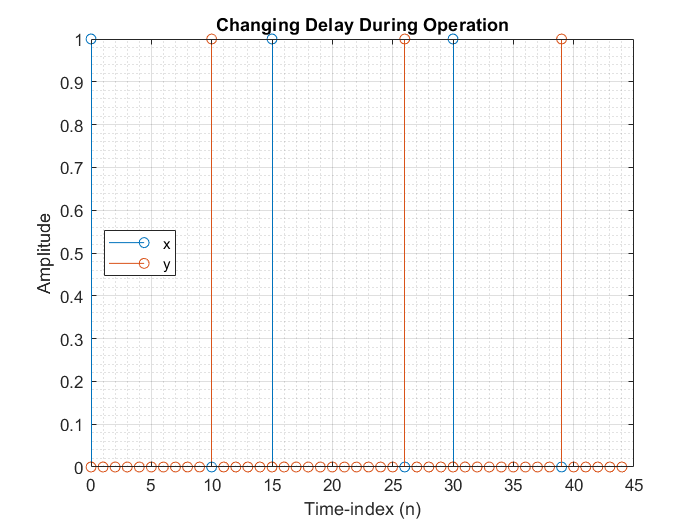
\includegraphics[scale=.65]{./images/plots/LagrangeTest2.png}
    \caption{$x[n]$ is an impulse train with a period of 15 samples and $y[n]$ represents the delay line output. The delay value starts at 10, increases to 11 at $n = 15$ and decreases to 9 at $n = 30$.}
    \label{fig:LagrangeTest2}
\end{figure}

The third test which was done is similar to the second, however now the fractional component was changed to ensure the coefficients of the Lagrange FIR are calculated correctly. Table~\ref{tab:LagrangeTest3} illustrates the parameter changes which occur every 15 samples. Under these conditions, the length of the interpolation filter is 6 samples, while $M$ is 8 samples. The output of this test is shown in Fig.~\ref{fig:LagrangeTest3}. As is clearly shown, the impulse response of the Lagrange interpolator, corresponding to the different fractional delays, appears in the six samples after the eight zeros (which correspond to the integer delay component of the structure).

\begin{figure}[h!]
    \centering
    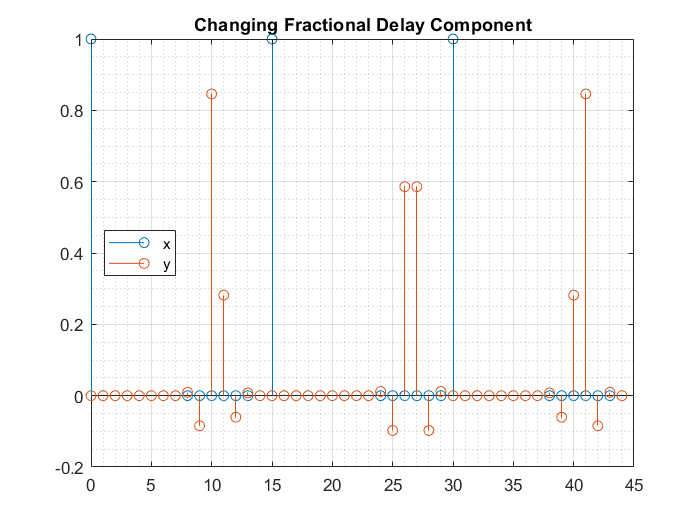
\includegraphics[scale=.65]{./images/plots/LagrangeTest3.png}
    \caption{$x[n]$ is an impulse train with a period of 15 samples used as input. $y[n]$ is the corresponding output. The parameter changes are specified in Table~\ref{tab:LagrangeTest3}. The output clearly illustrates the appropriate number of integer delay values followed by the impulse response of a filter approximating the Lagrange interpolation.}
    \label{fig:LagrangeTest3}
\end{figure}

\begin{table}[h!]
    \centering
     \begin{tabular}{||c| |c |c |c|} 
         \hline
         \textbf{n} & \textbf{M} & \textbf{d} & \textbf{D} \\ [0.5ex] 
         \hline
         0 & 8 & .25 & 10.25 \\ 
         \hline
         15 & 9 & .50 & 11.5 \\
         \hline
         30 & 8 & .75 & 10.75 \\
         \hline
    \end{tabular}
    \caption{Parameter changes for the test shown in Fig.\ref{fig:LagrangeTest3}}
    \label{tab:LagrangeTest3}
\end{table}

\subsection{Energy Scaler}
The energy scaling coefficient is governed by the following equation:
\begin{equation}
    g_c[n] = \sqrt{1-\Delta x[n]}
\end{equation}
where $\Delta x[n]$ is the change in the length of the digital waveguide, in samples, at time-step $n$. Testing of this block was done by specifying two different curves representing the digital waveguide length in samples over time. As $x[n]$ could take an infinite variety of different sorts of functions, it was decided to limit the curves to be linear and quadratic. The theoretical output of what the energy scaler should produce was derived and then the output error was calculated using the derived restuls.

Assuming we start with a continuous signal, a quadratic DWG length signal can be expressed as:
\begin{equation}
    DWGLength(t) = at^2 + c 
\end{equation}
Given $c = DWGLength(0)$,  the starting point of the sweep, then $a$ can be expressed as:
\begin{equation}
    a = \frac{sweepEnd - sweepStart}{sweepDuration^2}
\end{equation}
The continuous signal can then be sampled to produce the following discrete-time expressions:
\begin{align}
    DWGLength[n] = DWGLength(nT_s) = a(nT_s)^2 + c\\
    DWGLength[n-1] = a(n^2 - 2n + 1)T_s^2 + c
\end{align}
Given that $\Delta x = DWGLength[n] - DWGLength[n-1]$, we can express $g_c[n]$ as:
\begin{equation}
    g_c[n] = \sqrt{|1-a(2n-1)T_s^2|}
\end{equation}
and use the expressions for $a$ and $b$ to develop a parameterized theoretical curve for the ideal output to a quadratic input. A similar procedure can be followed for the simpler linear case.

Figure~\ref{fig:EnergyScalerLinInc} and Fig.~\ref{fig:EnergyScalerQuadInc} show the results for the linear and quadratic DWG Length functions respectively. The output to a linearly increasing function is a constant gain factor less than one. Intuitively this is what we would expect as the change in the DWG Length on a per sample basis is a constant value and the length of the DWG is increasing. It is necessary to attenuate the energy slightly as it spreads out across the new DWG Length. The output to a quadratically increasing function is a linearly decreasing function. Intuitively this makes sense as the change in length at each time step is gradually getting larger. It is necessary to attenuate the signal more and more to maintain the same perceptual loudness as the energy spreads out more across the length of the digital waveguide. 

Figure~\ref{fig:EnergyScalerLinDec} and Fig.~\ref{fig:EnergyScalerQuadDec} illustrate the output to the same functions which are now decreasing. As is illustrated, the error remains zero and the gain operates in the same pattern but applying amplification. Amplification is required in order to maintain the same perceptual loudness as samples are being discarded by the shortening length.

\begin{figure}[h!]
    \centering
    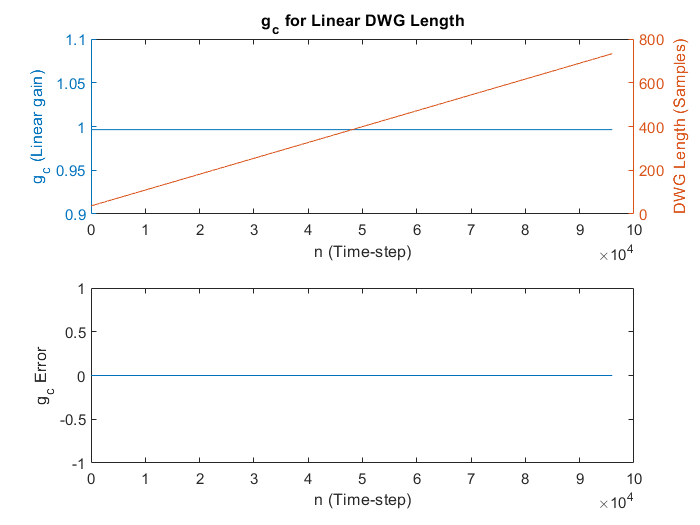
\includegraphics[scale=.50]{./images/plots/EnergyScalerLinearIncreasing.png}
    \caption{Energy scaler output for linearly increasing input}
    \label{fig:EnergyScalerLinInc}
\end{figure}

\begin{figure}[h!]
    \centering
    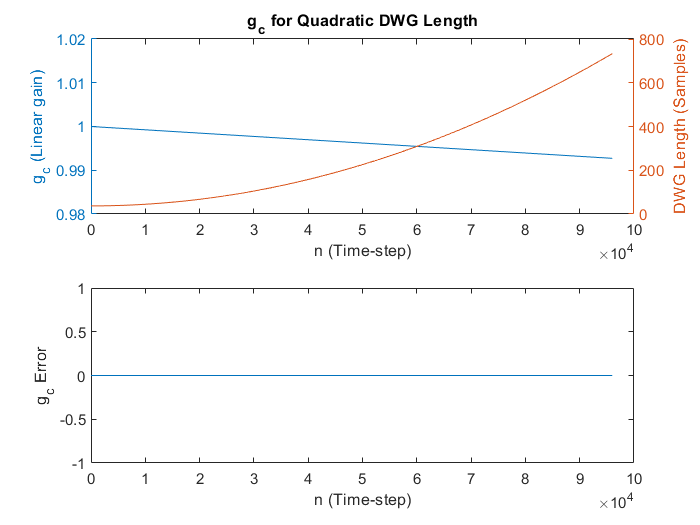
\includegraphics[scale=.50]{./images/plots/EnergyScalerQuadraticIncreasing.png}
    \caption{Energy scaler output for quadraticly increasing output}
    \label{fig:EnergyScalerQuadInc}
\end{figure}

\clearpage

\begin{figure}[h!]
    \centering
    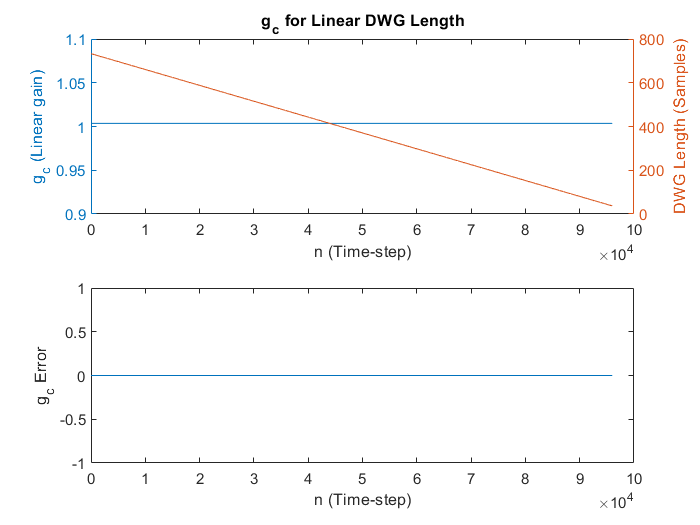
\includegraphics[scale=.63]{./images/plots/EnergyScalerLinearDecreasing.png}
    \caption{Energy scaler output for linearly decreasing input}
    \label{fig:EnergyScalerLinDec}
\end{figure}

\begin{figure}[h!]
    \centering
    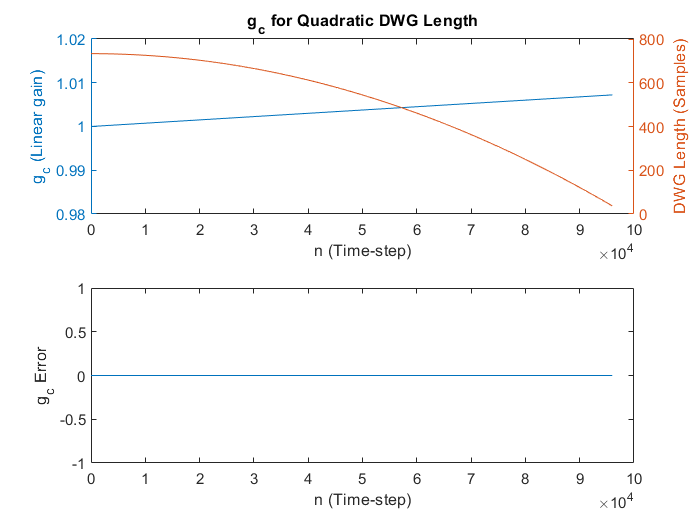
\includegraphics[scale=.63]{./images/plots/EnergyScalerQuadraticDecreasing.png}
    \caption{Energy scaler output for quadraticly decreasing output}
    \label{fig:EnergyScalerQuadDec}
\end{figure}

\clearpage

\subsection{String Digital Waveguide}
The string digital waveguide model was first verified to be transient and artifact free. This was achieved by running a series of sweeps across the range of valid relative length parameters. After this was ensured, the tuning accuracy was verified via parabolic spectral interpolation as outlined in \citetwo{smith_spectral_nodate}. This method relies taking the DFT of the signal to sample its spectrum at N evenly spaced, making them  harmonically related, analysis frequencies.

Ideally it would be best to have the harmonics generated by the string match the analysis frequencies. This would mitigate spectral leakage and reduce the need for interpolation in general. The fundamental frequency of the synthesized pitch was selected to align with a DFT bin but also be high enough so that several DFT bins exist in between the different harmonics. This is another method for mitigating spectral leakage. A lower fundamental frequency would produce a much more spectrally dense sound, which would be harder to get a clean estimate for.

The initial assumption in the algorithm development was that the strongest resonance present in the signal would be the fundamental frequency. In practice this was not the case, likely due to the initial waveform being initialized by noise as well as the non-idealities in the Loop Filter's magnitude response. The assumption had to be modified and the search range of the algorithm is limited $1.5*F_{0_{bin}}$, where $F_{0_{bin}}$ is the DFT bin associated with the synthesized sound. Other reasons for violations of the assumption could include the non-constant phase delay of both the loop as well as interpolation filter causing the frequencies to not all experience the same travel time and create a slight shift away from a perfectly harmonic signal.

To analyze the test the signal, the following STFT analysis parameters were used:
\begin{itemize}
    \item Window Type = Hamming
    \item $Fs = 48,000$ hz
    \item $N = 4096$
    \item Overlap = 75%
    \item Window length = 12 ms
\end{itemize}

The DWG was configured to generate a signal with a fundamental frequency corresponding with $F_{0_{bin}} = 100$, or 1,171.9 Hz. Following the method described in \citetwo{smith_spectral_nodate}, the calculated bin error was $8.3499 \times 10^{-5}$. In hertz this is $9.7850 \times 10^{-4}$. As this is extremely small, the tuning was considered to be accurate and verified. Figure~\ref{fig:DWGInterpBins}, Fig.~\ref{fig:DWGInterpBinsZoom} and Fig.~\ref{fig:DWGInterpSpec} illustrate this process.

\begin{figure}[h]
    \centering
    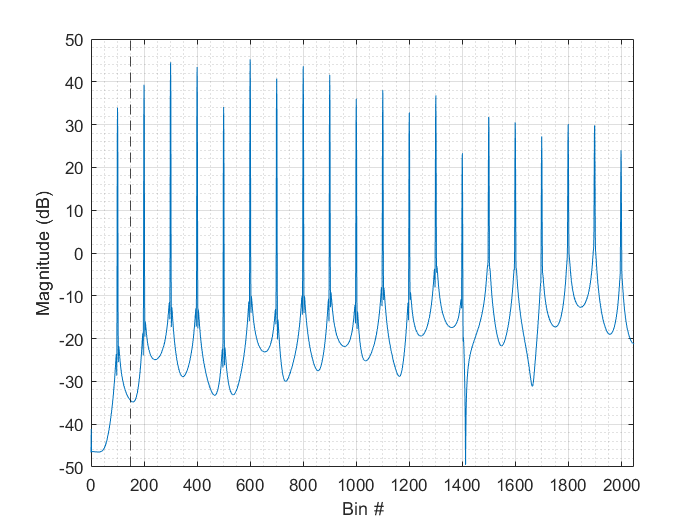
\includegraphics[scale=.65]{./images/plots/StringDWGInterpBins.png}
    \caption{FFT Spectrum of tone for tuning verification. note the upper harmonics which surpass the fundamental. The dashed-black line indicates the upper search limit.}
    \label{fig:DWGInterpBins}
\end{figure}

\begin{figure}[h!]
    \centering
    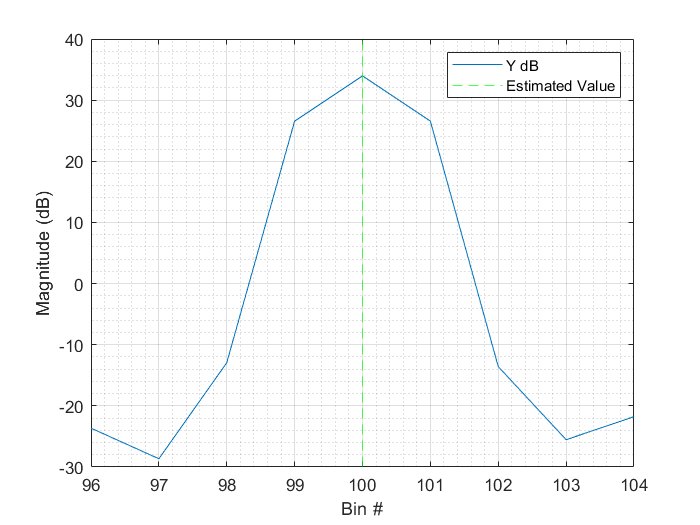
\includegraphics[scale=.58]{./images/plots/StringDWGInterpBinsZoom.png}
    \caption{Zoom of FFT for tuning verification.}
    \label{fig:DWGInterpBinsZoom}
\end{figure}

\begin{figure}[h!]
    \centering
    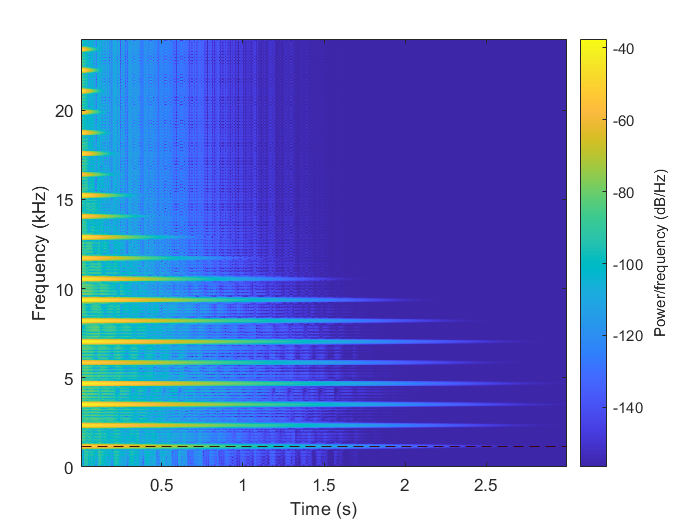
\includegraphics[scale=.58]{./images/plots/StringDWGInterpSpec.png}
    \caption{Tuning verification spectrum. Black-dashed line is estimation of fundamental.}
    \label{fig:DWGInterpSpec}
\end{figure}

% \clearpage

\section{Slide Synthesizer}
After all the individual components had been verified, a series of tests were run to check the overall functioning of the slide synthesizer. These tests were not meant to necessarily by physically accurate or musically useful, but purely as an approach to benchmark its basic behavior and determine the relationships between the CSG and DWG sound components. These were run with the different combinations of noise sources and harmonic accentuators as well as on the different string types. 

The testing scenarios are:
\begin{enumerate}
    \item Basic pluck with no slide motion
    \item Sliding up/down one fret over three seconds
    \item Sliding up/down three frets over one second
    \item Sliding up/down five frets over .5 seconds
    \item Sliding up/down extremes of relative string length
    \item Narrow/wide vibrato
\end{enumerate}
The output files and spectrograms were generated using the Noise Pulse Train and Harmonic Resonator Bank configuration using a mixture of the different strings. The filenames are \emph{SlideSynth-Test-\#-direction.wav}, where \emph{\#} is replaced with the corresponding test number and \emph{direction} is either up or down.

Figure~\ref{fig:VibratoWideSpec} and Fig.~\ref{fig:VibratoNarrowSpec} show the spectra from the different vibrato tests. As can clearly be seen, the harmonics follow a sinusoidal trajectory corresponding to the parameters of the specified vibrato. The variations in the contact sound intensity can be seen as well. As is also shown, the contact sound dominates the spectrum as the string dies out, which is similar to what happens in the physical world.

\begin{figure}[h!]
    \centering
    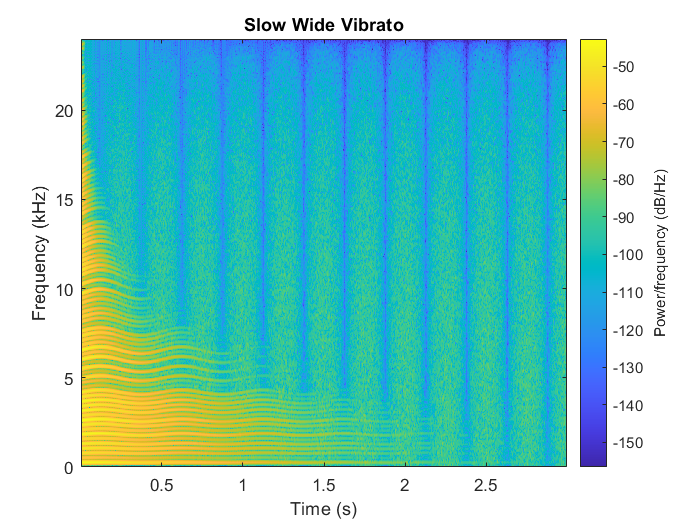
\includegraphics[scale=.65]{./images/plots/VibratoWideSpec.png}
    \caption{}
    \label{fig:VibratoWideSpec}
\end{figure}

\begin{figure}[h!]
    \centering
    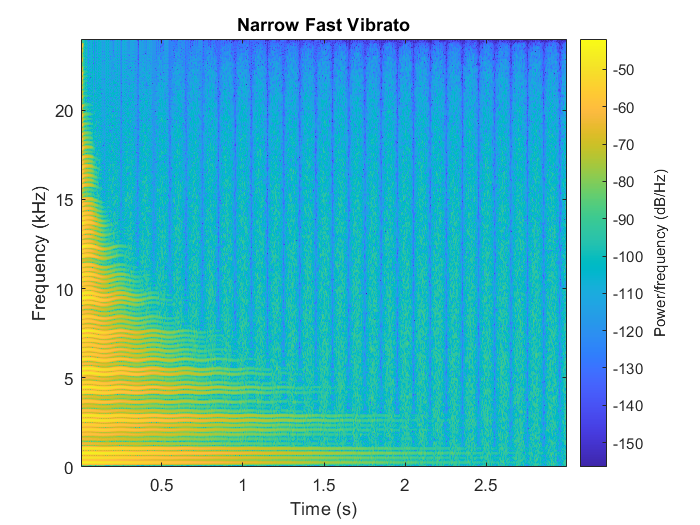
\includegraphics[scale=.65]{./images/plots/VibratoNarrowSpec.png}
    \caption{}
    \label{fig:VibratoNarrowSpec}
\end{figure}

\end{document}